\documentclass{ximera}
\graphicspath{  %% When looking for images,
{./}            %% look here first,
{./pictures/}   %% then look for a pictures folder,
{../pictures/}  %% which may be a directory up.
{../../pictures/}  %% which may be a directory up.
{../../../pictures/}  %% which may be a directory up.
{../../../../pictures/}  %% which may be a directory up.
}

\usepackage{listings}
%\usepackage{circuitikz}
\usepackage{xcolor}
\usepackage{amsmath,amsthm}
\usepackage{subcaption}
\usepackage{graphicx}
\usepackage{tikz}
%\usepackage{tikz-3dplot}
\usepackage{amsfonts}
%\usepackage{mdframed} % For framing content
%\usepackage{tikz-cd}

  \renewcommand{\vector}[1]{\left\langle #1\right\rangle}
  \newcommand{\arrowvec}[1]{{\overset{\rightharpoonup}{#1}}}
  \newcommand{\ro}{\texttt{R}}%% row operation
  \newcommand{\dotp}{\bullet}%% dot product
  \renewcommand{\l}{\ell}
  \let\defaultAnswerFormat\answerFormatBoxed
  \usetikzlibrary{calc,bending}
  \tikzset{>=stealth}
  




%make a maroon color
\definecolor{maroon}{RGB}{128,0,0}
%make a dark blue color
\definecolor{darkblue}{RGB}{0,0,139}
%define the color fourier0 to be the maroon color
\definecolor{fourier0}{RGB}{128,0,0}
%define the color fourier1 to be the dark blue color
\definecolor{fourier1}{RGB}{0,0,139}
%define the color fourier 1t to be the light blue color
\definecolor{fourier1t}{RGB}{173,216,230}
%define the color fourier2 to be the dark green color
\definecolor{fourier2}{RGB}{0,100,0}
%define teh color fourier2t to be the light green color
\definecolor{fourier2t}{RGB}{144,238,144}
%define the color fourier3 to be the dark purple color
\definecolor{fourier3}{RGB}{128,0,128}
%define the color fourier3t to be the light purple color
\definecolor{fourier3t}{RGB}{221,160,221}
%define the color fourier0t to be the red color
\definecolor{fourier0t}{RGB}{255,0,0}
%define the color fourier4 to be the orange color
\definecolor{fourier4}{RGB}{255,165,0}
%define the color fourier4t to be the darker orange color
\definecolor{fourier4t}{RGB}{255,215,0}
%define the color fourier5 to be the yellow color
\definecolor{fourier5}{RGB}{255,255,0}
%define the color fourier5t to be the darker yellow color
\definecolor{fourier5t}{RGB}{255,255,100}
%define the color fourier6 to be the green color
\definecolor{fourier6}{RGB}{0,128,0}
%define the color fourier6t to be the darker green color
\definecolor{fourier6t}{RGB}{0,255,0}

%New commands for this doc for errors in copying
\newcommand{\eigenvar}{\lambda}
%\newcommand{\vect}[1]{\mathbf{#1}}
\renewcommand{\th}{^{\text{th}}}
\newcommand{\st}{^{\text{st}}}
\newcommand{\nd}{^{\text{nd}}}
\newcommand{\rd}{^{\text{rd}}}
\newcommand{\paren}[1]{\left(#1\right)}
\newcommand{\abs}[1]{\left|#1\right|}
\newcommand{\R}{\mathbb{R}}
\newcommand{\C}{\mathbb{C}}
\newcommand{\Hilb}{\mathbb{H}}
\newcommand{\qq}[1]{\text{#1}}
\newcommand{\Z}{\mathbb{Z}}
\newcommand{\N}{\mathbb{N}}
\newcommand{\q}[1]{\text{``#1''}}
%\newcommand{\mat}[1]{\begin{bmatrix}#1\end{bmatrix}}
\newcommand{\rref}{\text{reduced row echelon form}}
\newcommand{\ef}{\text{echelon form}}
\newcommand{\ohm}{\Omega}
\newcommand{\volt}{\text{V}}
\newcommand{\amp}{\text{A}}
\newcommand{\Seq}{\textbf{Seq}}
\newcommand{\Poly}{\textbf{P}}
\renewcommand{\quad}{\text{    }}
\newcommand{\roweq}{\simeq}
\newcommand{\rowop}{\simeq}
\newcommand{\rowswap}{\leftrightarrow}
\newcommand{\Mat}{\textbf{M}}
\newcommand{\Func}{\textbf{Func}}
\newcommand{\Hw}{\textbf{Hamming weight}}
\newcommand{\Hd}{\textbf{Hamming distance}}
\newcommand{\rank}{\text{rank}}
\newcommand{\longvect}[1]{\overrightarrow{#1}}
% Define the circled command
\newcommand{\circled}[1]{%
  \tikz[baseline=(char.base)]{
    \node[shape=circle,draw,inner sep=2pt,red,fill=red!20,text=black] (char) {#1};}%
}

% Define custom command \strikeh that just puts red text on the 2nd argument
\newcommand{\strikeh}[2]{\textcolor{red}{#2}}

% Define custom command \strikev that just puts red text on the 2nd argument
\newcommand{\strikev}[2]{\textcolor{red}{#2}}

%more new commands for this doc for errors in copying
\newcommand{\SI}{\text{SI}}
\newcommand{\kg}{\text{kg}}
\newcommand{\m}{\text{m}}
\newcommand{\s}{\text{s}}
\newcommand{\norm}[1]{\left\|#1\right\|}
\newcommand{\col}{\text{col}}
\newcommand{\sspan}{\text{span}}
\newcommand{\proj}{\text{proj}}
\newcommand{\set}[1]{\left\{#1\right\}}
\newcommand{\degC}{^\circ\text{C}}
\newcommand{\centroid}[1]{\overline{#1}}
\newcommand{\dotprod}{\boldsymbol{\cdot}}
%\newcommand{\coord}[1]{\begin{bmatrix}#1\end{bmatrix}}
\newcommand{\iprod}[1]{\langle #1 \rangle}
\newcommand{\adjoint}{^{*}}
\newcommand{\conjugate}[1]{\overline{#1}}
\newcommand{\eigenvarA}{\lambda}
\newcommand{\eigenvarB}{\mu}
\newcommand{\orth}{\perp}
\newcommand{\bigbracket}[1]{\left[#1\right]}
\newcommand{\textiff}{\text{ if and only if }}
\newcommand{\adj}{\text{adj}}
\newcommand{\ijth}{\emph{ij}^\text{th}}
\newcommand{\minor}[2]{M_{#2}}
\newcommand{\cofactor}{\text{C}}
\newcommand{\shift}{\textbf{shift}}
\newcommand{\startmat}[1]{
  \left[\begin{array}{#1}
}
\newcommand{\stopmat}{\end{array}\right]}
%a command to give a name to explorations and hints and theorems
\newcommand{\name}[1]{\begin{centering}\textbf{#1}\end{centering}}
\newcommand{\vect}[1]{\vec{#1}}
\newcommand{\dfn}[1]{\textbf{#1}}
\newcommand{\transpose}{\mathsf{T}}
\newcommand{\mtlb}[2][black]{\texttt{\textcolor{#1}{#2}}}
\newcommand{\RR}{\mathbb{R}} % Real numbers
\newcommand{\id}{\text{id}}
\newcommand{\coord}[1]{\langle#1\rangle}
\newcommand{\RREF}{\text{RREF}}
\newcommand{\Null}{\text{Null}}
\newcommand{\Nullity}{\text{Nullity}}
\newcommand{\Rank}{\text{Rank}}
\newcommand{\Col}{\text{Col}}
\newcommand{\Ef}{\text{EF}}
\newcommand{\boxprod}[3]{\abs{(#1\times#2)\cdot#3}}

\author{Zack Reed}
%borrowed from selinger linear algebra
\title{Singular Value Decomposition (SVD): Rotations and Stretches}
\begin{document}
\begin{abstract}

\end{abstract}
\maketitle

\section*{Introduction: Matrix Decompositions}
In previous sections we've spent much time multiplying matrices together to form single matrices representing the emalgumation of the transformations from each matrix in the product. 

For instance, the matrix $A=\begin{bmatrix} 2 & -1 \\ 3 & 0\end{bmatrix}$ is the product of a $90^\circ$ rotation matrix $\begin{bmatrix}0 & -1\\ 1 & 0\end{bmatrix}$, a shear $\begin{bmatrix} 1 & 2 \\ 0 & 1\end{bmatrix}$ and a vertical stretch $\begin{bmatrix} 1 & 0 \\ 0 & 3\end{bmatrix}$. We're cheating a little bit since we know how $A$ was built, but we could say that $A$ can be \emph{decomposed} into three matrices via the product 

$$\begin{bmatrix} 2 & -1 \\ 3 & 0\end{bmatrix}=\begin{bmatrix} 1 & 0 \\ 0 & 3\end{bmatrix}*\begin{bmatrix} 1 & 2 \\ 0 & 1\end{bmatrix}*\begin{bmatrix}0 & -1\\ 1 & 0\end{bmatrix}.$$

You can check this effect by transforming points by the matrix $A$, such as the points in \texttt{+linalg/face\_points.mat} via

\begin{verbatim}

  load +linalg/face_points.mat
  rotate_1=[cos(pi/2) -sin(pi/2);
    sin(pi/2) cos(pi/2)]
  shear_1=[1 2;
      0 1]
  stretch_y=[1 0;
      0 3]
  A=stretch_y*shear_1*rotate_1
  trans_face=A*face_points
  linalg.simple_plot_cloud(trans_face);

\end{verbatim}

which yields the following figure 

%1120x840
\begin{center}
  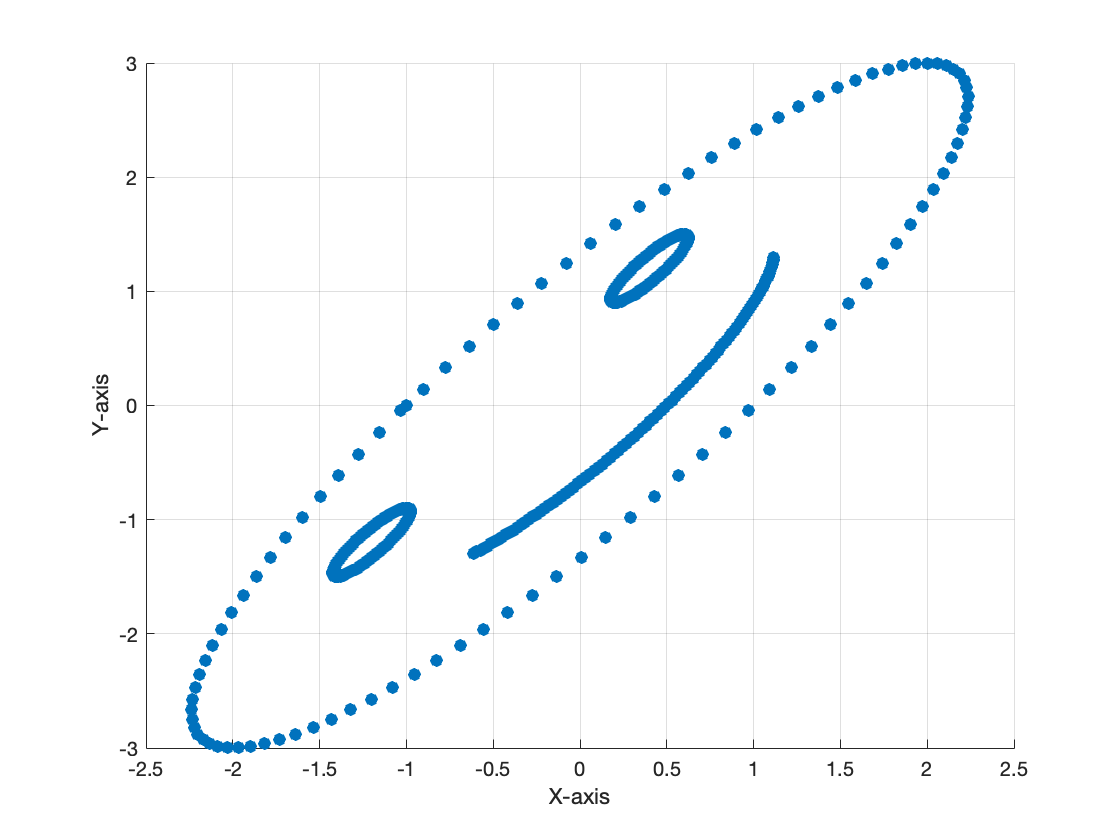
\includegraphics[width=29.63cm, height=22.22cm]{face_svd_intro_A.png}
\end{center}

If you then individually apply the transformations to \texttt{face\_points}, you should yeild the same figure. 

We also spent a considerable amount of time finding inverse matrices as products of elementary matrices via Gaussian Elimination. For instance, if we reverse the transformations (i.e. find the inverse of each transformation) we then get the inverse matrix $A^{-1}$.

Reversing a vertical stretch is the vertical compression $\begin{bmatrix}1 &0\\
  0 &1/3\end{bmatrix}$ which yields

  \begin{verbatim}

    reverse_face=[1 0;0 1/3]*trans_face
    linalg.simple_plot_cloud(reverse_face);

  \end{verbatim}

  %1120x840
\begin{center}
  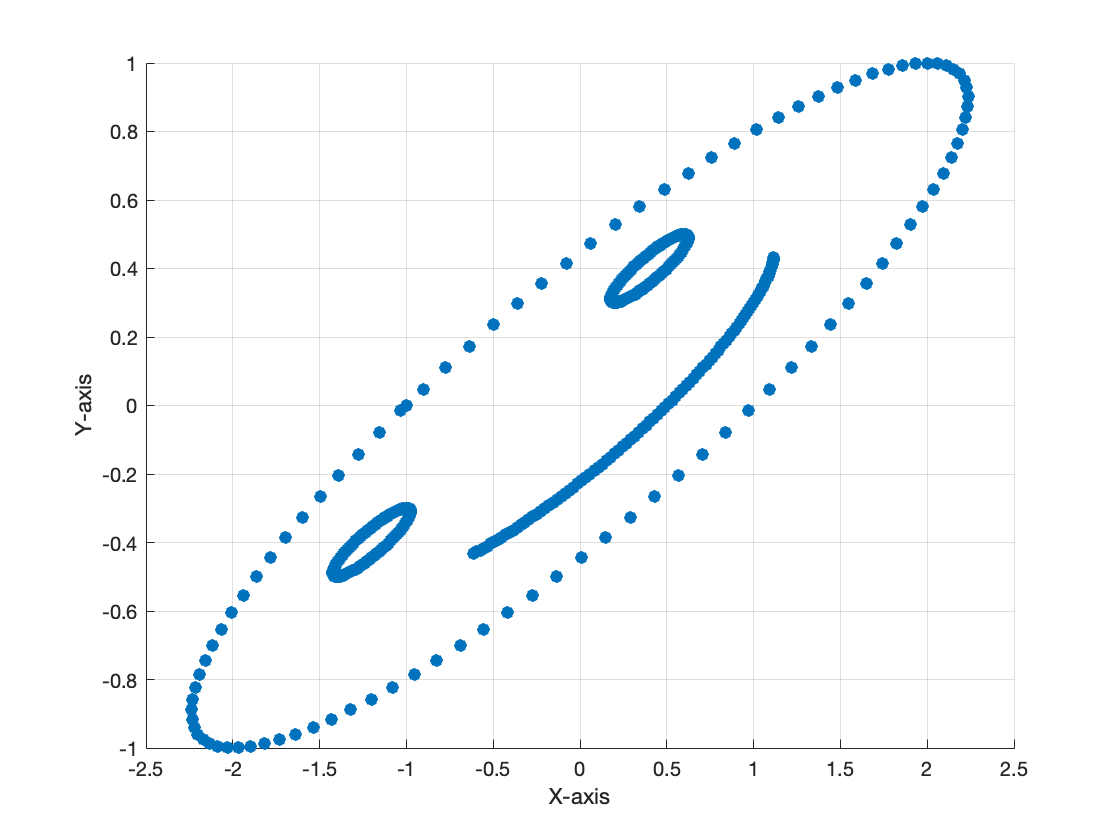
\includegraphics[width=29.63cm, height=22.22cm]{face_svd_intro_A_reverse_1.png}
\end{center}

then you un-do the shear by shearing in the reverse direction $\begin{bmatrix}1 &-2\\
  0 &1\end{bmatrix}$ which yields 

  \begin{verbatim}

    reverse_face=[1 -2;0 1]*reverse_face
    linalg.simple_plot_cloud(reverse_face);

  \end{verbatim}

  %1120x840
\begin{center}
  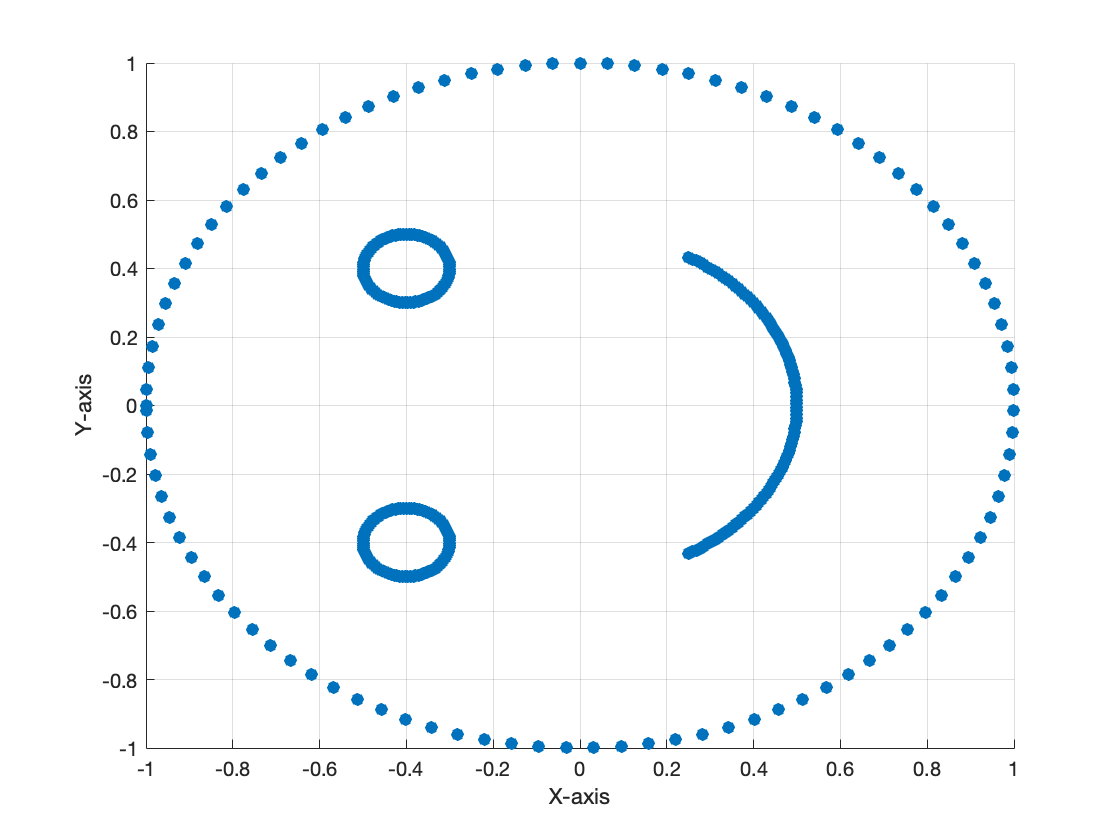
\includegraphics[width=29.63cm, height=22.22cm]{face_svd_intro_A_reverse_2.png}
\end{center}

and then you un-do the rotation by rotating in the reverse direction $\begin{bmatrix}\cos(-\pi/2) & -\sin(-\pi/2)\\
  \sin(-\pi/2) & \cos(-\pi/2)\end{bmatrix}$,

  \begin{verbatim}

    reverse_face=[0 -1;-1 0]*reverse_face
    linalg.simple_plot_cloud(reverse_face);

  \end{verbatim}

which yields the original face.

This means that we have a decomposition of $A^{-1}$ as 
$$\begin{bmatrix}\cos(-\pi/2) & -\sin(-\pi/2)\\\sin(-\pi/2) & \cos(-\pi/2)\end{bmatrix}*\begin{bmatrix}1 &-2\\0 &1\end{bmatrix}*\begin{bmatrix}1 &0\\0 &1/3\end{bmatrix}=\begin{bmatrix}0 & 1/3\\-1 & 2/3\end{bmatrix}.$$

Important data analysis techniques arising from Linear Algebra recreate this process of \emph{decomposition}, but start with a matrix for which we don't know the decomposition and end with the product of two or more matrices that make up the matrix. This would be akin to starting with $A$, performing some Linear Algebra manipulations on $A$, and ending up with the otherwise unknown matrices $\begin{bmatrix} 1 & 0 \\ 0 & 3\end{bmatrix}$, $\begin{bmatrix} 1 & 2 \\ 0 & 1\end{bmatrix}$, and $\begin{bmatrix}0 & -1\\ 1 & 0\end{bmatrix}$. 


The analysis on voting records in \href{https://ximera.osu.edu/appliedlinearalgebra/c6ChapterSix/learningActivities/m6LearningActivities/leastSquares/leastSquaresApplicationVotingImages}{the previous section} can be performed through a special matrix decomposition called the \emph{singular value decomposition}. This particular decomposition forms the backbone of many modern data analysis techniques, and is at times the first step one takes when buildling machine learlning models today. The \emph{singular value decomposition} (SVD) is also useful in engineering, the sciences, and many software-based applications. We will be using the SVD as a context in which to unpack many important ideas in Linear Algebra.

In many mathematics texts, you spend the majority of your time learning how to \emph{compute} something, often by hand, and then only later do you learn \emph{why} you might make a computation or \emph{how} a computation can be used for various tasks. Hopefully this somewhat different introduction to the SVD accompanies some intuition about why the computation works the way it does. 

As you move beyond this course, however, and especially once you progress into your specific domains of study (engineering, data science, etc.), you will increasingly rely on technology to perform computations for you and your primary job is to know \emph{when} to make a computation, to \emph{interpret} the result of that computation, and to know \emph{what went wrong or right} when a computation yielded an unexpected result. 

We will foreground this latter approach to learning the SVD. In many respects, we have already been employing these emphases already, but this focus will be especially true for the SVD as we will gain a general understanding of one method of SVD computation at the very end of this chapter, and then gain other more employable computations in later chapters, but will largely spend our time: learning \emph{what} the SVD is, learning \emph{how} to use it in various situations, and using technology to calculate it for us.

\section*{SVD Part 1: ``Rotations" and Stretches}

The first important aspect of the SVD is that it decomposes \emph{any} matrix $M$ into three matrices, often called $U$, $S$, and $V$ (though you can label these matrices whatever you want). This is a very important utility of the SVD, that it works on any matrix. Many other useful decompositions only work on certain matrices with special conditions.

Let's explore the properties of these $U$, $S$, and $V$ matrices by re-examining our original matrix $A=\begin{bmatrix} 2 & -1 \\ 3 & 0\end{bmatrix}$.

The following video walks you through the main ideas of the next example.

\begin{center}
  \youtube{UjgCtmHSBHw}
\end{center}

To find the SVD in MATLAB, use the syntax \texttt{[U, S, V]=svd(A)}. \texttt{svd()} is one of those functions that gives multiple outputs, so if you don't list and name each output it will only return the first output (in this case the $U$ matrix). (Note: Sometimes you'll see $V$ denoted as $V^\dagger$ and $S$ denoted as $\Sigma$ we will just use $S$ and $V$)

The decomposition is that $A=U*S*V^{T}$. 



\begin{problem}
Let's use MATLAB to explore the properties of $U, S$, and $V$. Use \texttt{face\_points} as a test subject for the transformations associated with $U$, $S$, and $V$.


First, let's examine the transformational interpretations of the SVD first. In short, the SVD lets you write any matrix as the product of \emph{two ``rotations"} and a \emph{stretching}. This is much simpler than breaking down a matrix into elementary transformations, and even will work on matrices representing many transformations. (Note: We say ``rotations'' in quotes because in $2$ and $3$ dimensions these matrices could be a mix of rotations and reflections. More generally these are called \emph{orthogonal} matrices, which we'll explore later.)


  

  Trying this out on our $A$ matrix, we get $V^T=\begin{bmatrix}
    -.9871 & .1602 \\ .1602 & .9871
  \end{bmatrix}$. If we apply this to \texttt{face\_points}  with

  \begin{verbatim}
    new_face=V'*face_points
    linalg.simple_plot_cloud(new_face);
  \end{verbatim}

  we get the image

    %1120x840
    \begin{center}
      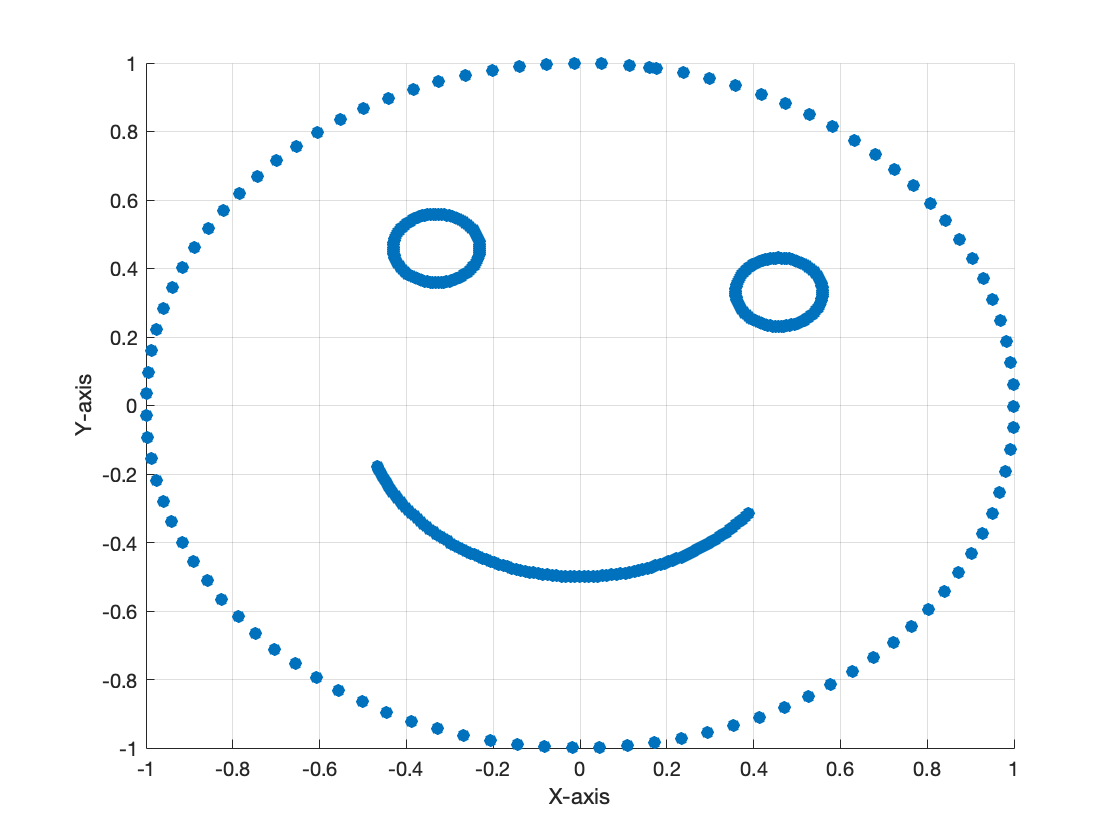
\includegraphics[width=29.63cm, height=22.22cm]{face_svd_rots_V_A.png}
    \end{center}

  Notice that this is a rotation of \texttt{face\_points} , but a different rotation than the construction rotation from the introduction.

  Applying what we know about orthogonal projections, the matrix $V^T$ has projected the face vectors to the orthonormal basis:

  

  $$v_1=\begin{bmatrix}\answer[tolerance=.001]{-.9871}\\\answer[tolerance=.0001]{.1602}\end{bmatrix}, v_2=\begin{bmatrix}\answer[tolerance=.001]{.1602}\\\answer[tolerance=.0001]{.9871}\end{bmatrix}. \text{ (Note: Answer these to four decimal places)}$$

  \begin{feedback}
    If you need to, it might help to use \texttt{linalg.simple\_plot\_quiver(V(1,:)',V(2,:)')} to visualize the the rotation with respect to the columns of $V$.

    The full code would be


    \begin{verbatim}
      A=[2 -1;3 0]
      [U, S, V]=svd(A)
      new_face=V'*face_points
      linalg.simple_plot_cloud(new_face);
      hold on
      linalg.simple_plot_quiver(V(:,1),V(:,2))
      hold off
    \end{verbatim}
  \end{feedback}

  
  Next, apply $S$ to $V^T*face\_points$

  \begin{verbatim}
    new_face=S*new_face
    linalg.simple_plot_cloud(new_face);
  \end{verbatim}

  we get the image

    %1120x840
    \begin{center}
      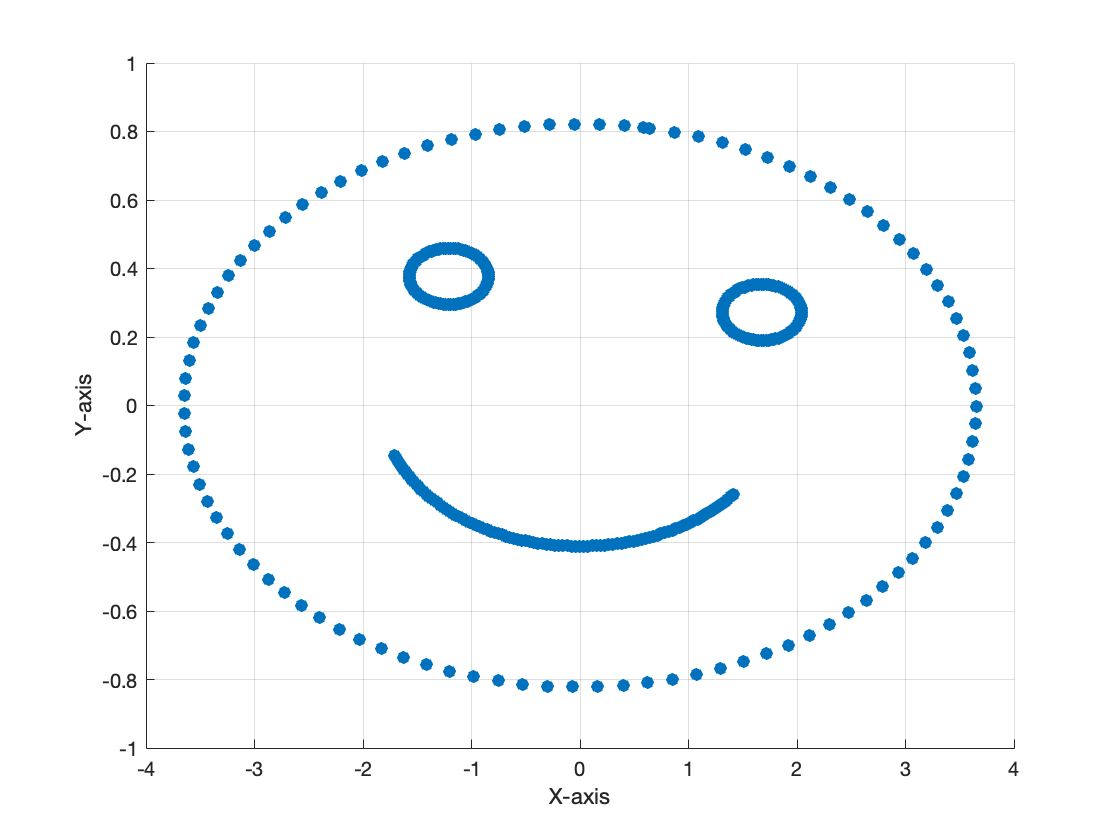
\includegraphics[width=29.63cm, height=22.22cm]{face_svd_rots_S_A.png}
    \end{center}

  Checking the dimensions of the new figure window, we notice that the face has compressed vertically inward and stretched horizontally outward, according to the diagonal values of $S$.

  Looking at the matrix $S$ the face is horizontally stretched by a factor of $\answer[tolerance=.01]{3.65}$ and horizontally compressed by a factor of $\answer[tolerance=.01]{.82}$.

  Finally, if we apply $U$ to $S*V'*$\texttt{face\_points}, we get 

  \begin{verbatim}
    new_face=U*new_face
    linalg.simple_plot_cloud(new_face);
  \end{verbatim}

  we get the same figure as when we apply $A$ to \texttt{face\_points} . 

  Keeping in mind the dimensions of the face image after multiplication by $S$, you'll note that $U$ applied another rotation. 

  This rotation aligns the face with the direction vectors $u_1=\begin{bmatrix}\answer[tolerance=.001]{-.5847}\\\answer[tolerance=.0001]{-.8112}\end{bmatrix}$ and $u_2=\begin{bmatrix}\answer[tolerance=.001]{-.8112}\\\answer[tolerance=.0001]{.5847}\end{bmatrix}$.


Connecting the ideas from last chapter about dot products and orthonormal bases, you might note that any rotation matrix in $\RR^2$ simply rotates the standard basis vectors while keeping them length 1 and orthogonal. One might conclude that any rotation in $\RR^2$ is given by an orthonormal basis for $\RR^2$. 

We have two rotation matrices here, let's check if they give orthonormal bases for $\RR^2$!

The dot products 

%V'*V gives the identity matrix and so does U'*U
$$V^T*V=\begin{bmatrix}\answer{1} & \answer{0}\\\answer{0} & \answer{1}\end{bmatrix} \text{ and } U^T*U=\begin{bmatrix}\answer{1} & \answer{0}\\\answer{0} & \answer{1}\end{bmatrix}.$$

Hence, $V$ and $U$ \wordChoice{\choice[correct]{give}\choice{do not give}} orthonormal bases for $\RR^2$.

Let's put this all together to determine the properties of $U$, $S$, and $V$!

\begin{selectAll}

  \choice[correct]{$V$ is a rotation matrix.}
  \choice{$U$ represents a shear transformation.}
  \choice[correct]{$S$ is a diagonal matrix.}
  \choice{$S$ swaps the coordinate axes.}
  \choice[correct]{The columns of $U$ are all unit vectors.}
  \choice{$U$ maps vectors into the null space of $A$.}
  \choice{$V$ maps vectors into the column space of $A$.}
  \choice{$V$ translates the rows of $A$ to a new origin.}
  \choice[correct]{$U$ is a rotation matrix.}
  \choice{$U$ scales the columns of $A$ by the diagonal of $S$ values.}
  \choice{$V$ is an upper triangular matrix.}
  \choice[correct]{The columns of $V$ are all unit vectors.}
  \choice[correct]{$S$ stretches and compresses along the coordinate axes.}
  \choice{$S$ represents a projection onto the row space of $A$.}
  \choice{$U$ permutes the rows of $A$.}
  \choice{$U*S*V$ also equals $A$.}
  \choice{$V$ flips the sign of all elements in $A$.}

\end{selectAll}

\end{problem}



As we said before, the SVD can be applied to \emph{any} matrix, unlike many decompositions that require square matrices. Let's again explore the SVD, but on two matrices that map $3$-dimensional vectors and are not full rank.

We'll first examine a rank 2 3x3 matrix, and then a 3x2 matrix, as these both will illuminate some important structural aspects of the SVD matrices. 

The following video walks you through the next example.

\begin{center}
  \youtube{HvqCC997pC8}
\end{center}

First, consider $B=\begin{bmatrix}1&3&-3\\0&1&-2\\1&-3&9\end{bmatrix}$. A quick use of \texttt{rref(B)} or \texttt{rank(B)} indeed confirms the rank of 2. 

We can further note the rank of $B$ by observing its effect on a $3$D cloud of vectors, say \texttt{+linalg/smiley\_3D.mat}. 

\begin{verbatim}

  B=[1 3 -3;
      0 1 -2;
      1 -3 9]
  load +linalg/smiley_3D.mat
  linalg.simple_plot_cloud(head, eyes, smile);
  face=[head,eyes,smile]
  two_face=B*face
  linalg.simple_plot_cloud(two_face);
\end{verbatim}

which yeilds the plots 

%1120x840
\begin{center}
  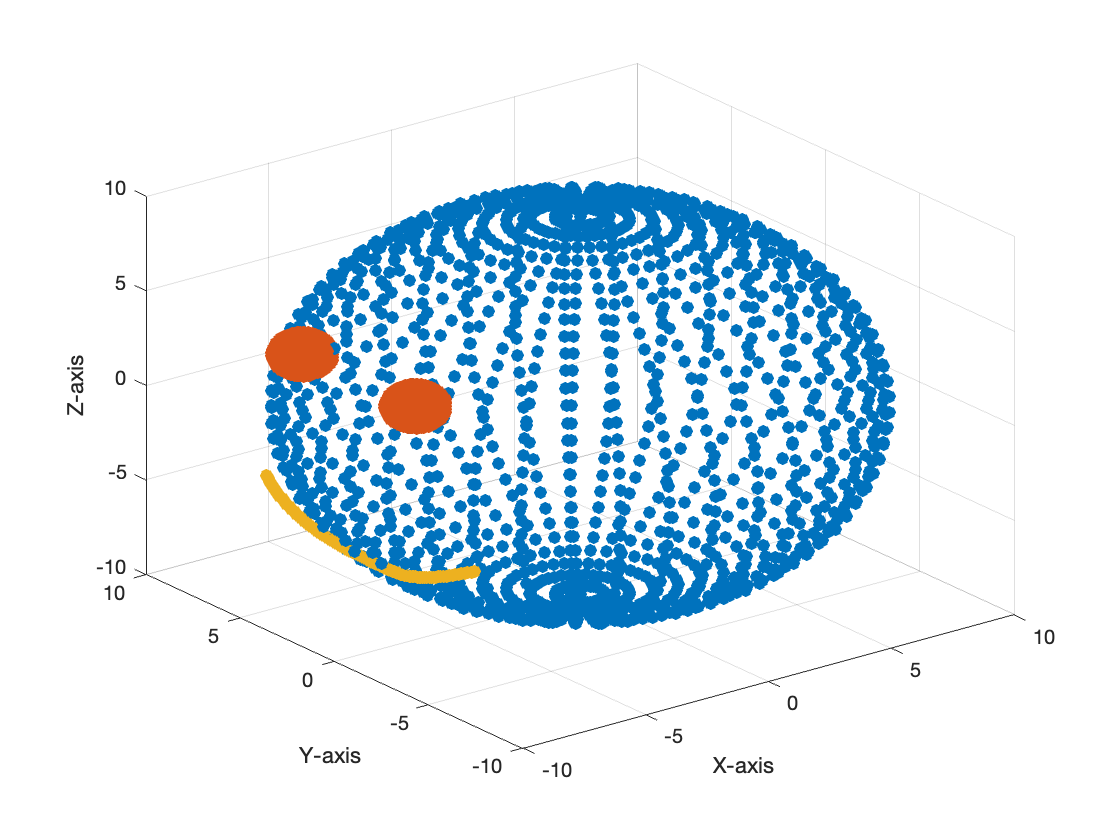
\includegraphics[width=29.63cm, height=22.22cm]{face_svd_3D.png}
\end{center}

    and 

%1120x840
\begin{center}
  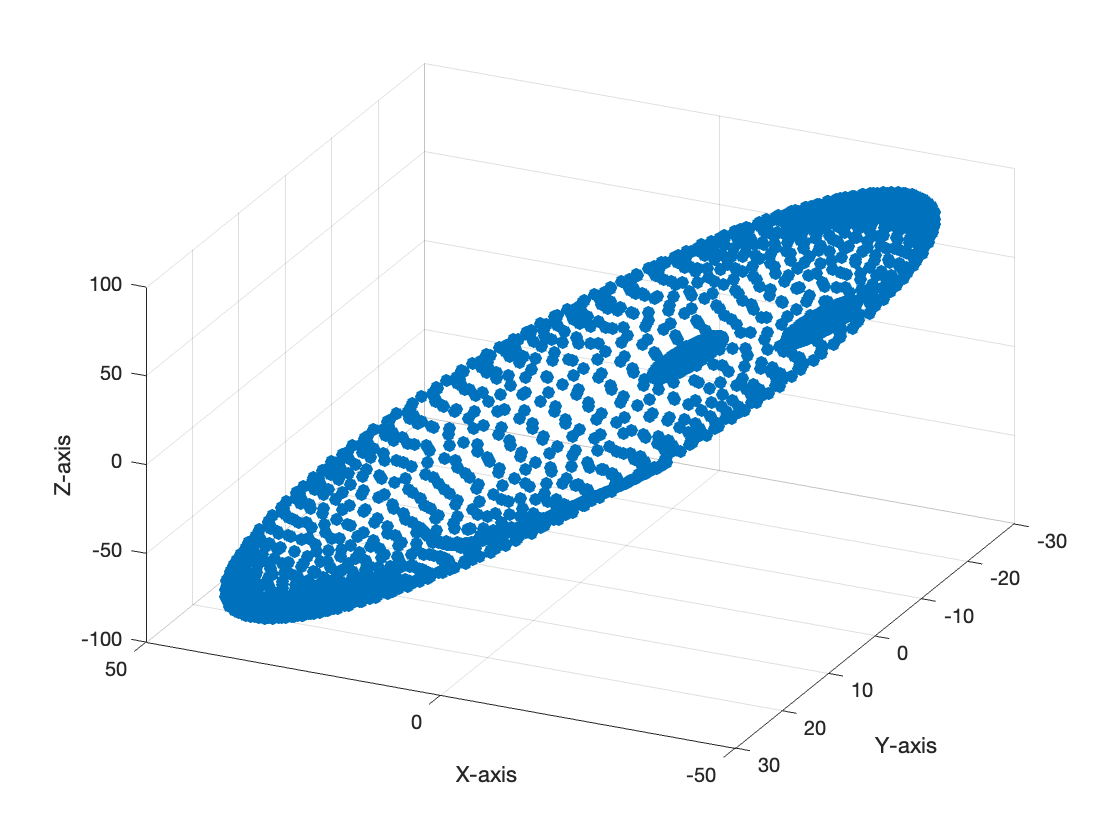
\includegraphics[width=29.63cm, height=22.22cm]{face_svd_3D_B_2D.png}
\end{center}

This visualizes more specifically the structure of $B$ in that it compresses space down to a plane. While further analysis of $B$ can determine which vectors span the image space, we can actually determine this same information from the SVD. 

\begin{problem}

First, remember that the SVD breaks down any matrix into two rotations and a stretch. Let's see these in action.

After taking the SVD, we start with the matrix $V_B^T$.

\begin{verbatim}

  [U_B, S_B, V_B]=svd(B)
  two_face=V_B'*face
  linalg.simple_plot_cloud(two_face)

\end{verbatim}

which yields

%1120x840
\begin{center}
  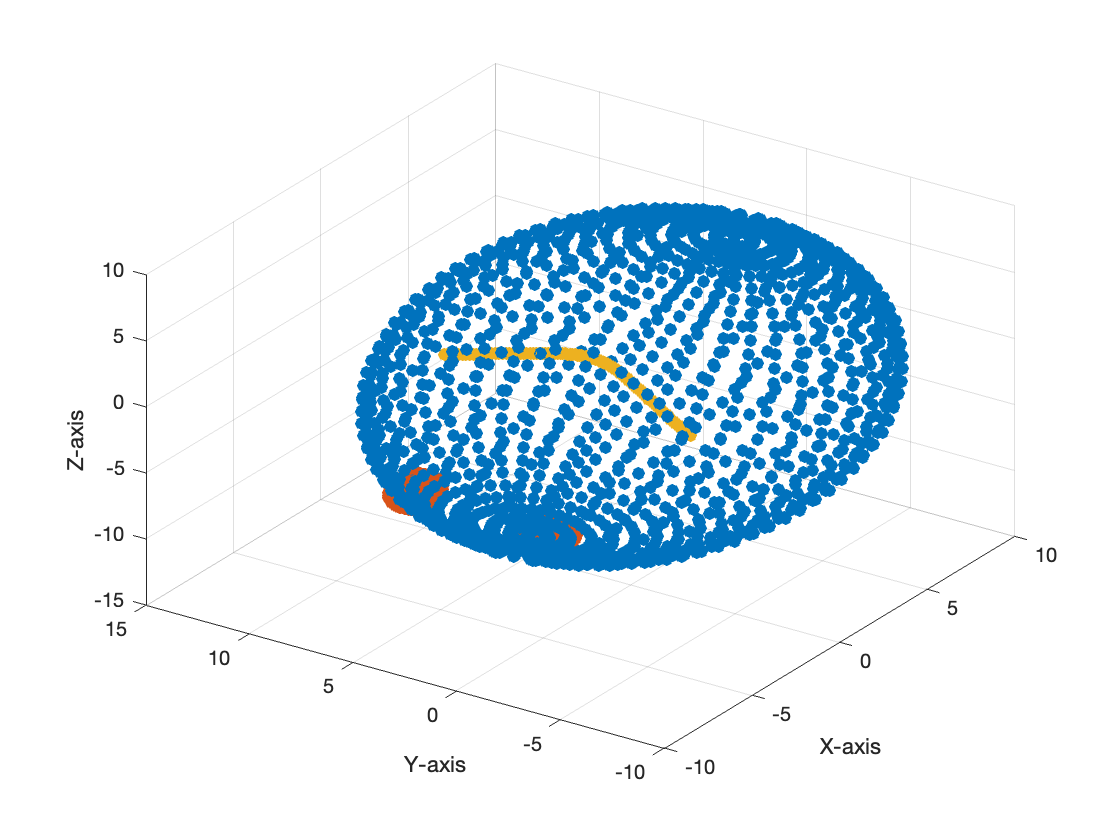
\includegraphics[width=29.63cm, height=22.22cm]{face_svd_3D_B_V.png}
\end{center}

(Note: I maintained the head, eyes, and smile separately for these figures so that the rotations were more evident.). This clearly performed a rotation in space, though the rotation was not over one specific axis of rotation, sucha as the standard rotations around the $x$, $y$, and $z$ axes.

The matrix $V'$ projected the face vectors along the orthonormal basis vectors: 

$$v_1=\begin{bmatrix}\answer[tolerance=.001]{-.0511}\\\answer[tolerance=.0001]{.3842}\\\answer[tolerance=.0001]{-.9218}\end{bmatrix}, v_2=\begin{bmatrix}\answer[tolerance=.001]{-.5954}\\\answer[tolerance=.0001]{-.7528}\\\answer[tolerance=.0001]{-.2807}\end{bmatrix}, v_3=\begin{bmatrix}\answer[tolerance=.001]{.8018}\\\answer[tolerance=.0001]{-.5345}\\\answer[tolerance=.0001]{-.2673}\end{bmatrix}.$$

\begin{feedback}
To visualize this orientation along the new axis, use the following code (in addition to the previous code). Note that the scaling factors are arbitrary and can be adjusted to better visualize the vectors.

\begin{verbatim}
  hold on
  linalg.simple_plot_quiver(10*V_B(1,:)',10*V_B(2,:)',10*V_B(3,:)');
  hold off
\end{verbatim}

\end{feedback}

Then, we follow up by multiplying by $S_B$.

\begin{verbatim}

  two_face=S_B*two_face
  linalg.simple_plot_cloud(two_face);

\end{verbatim}

which yields

%1120x840
\begin{center}
  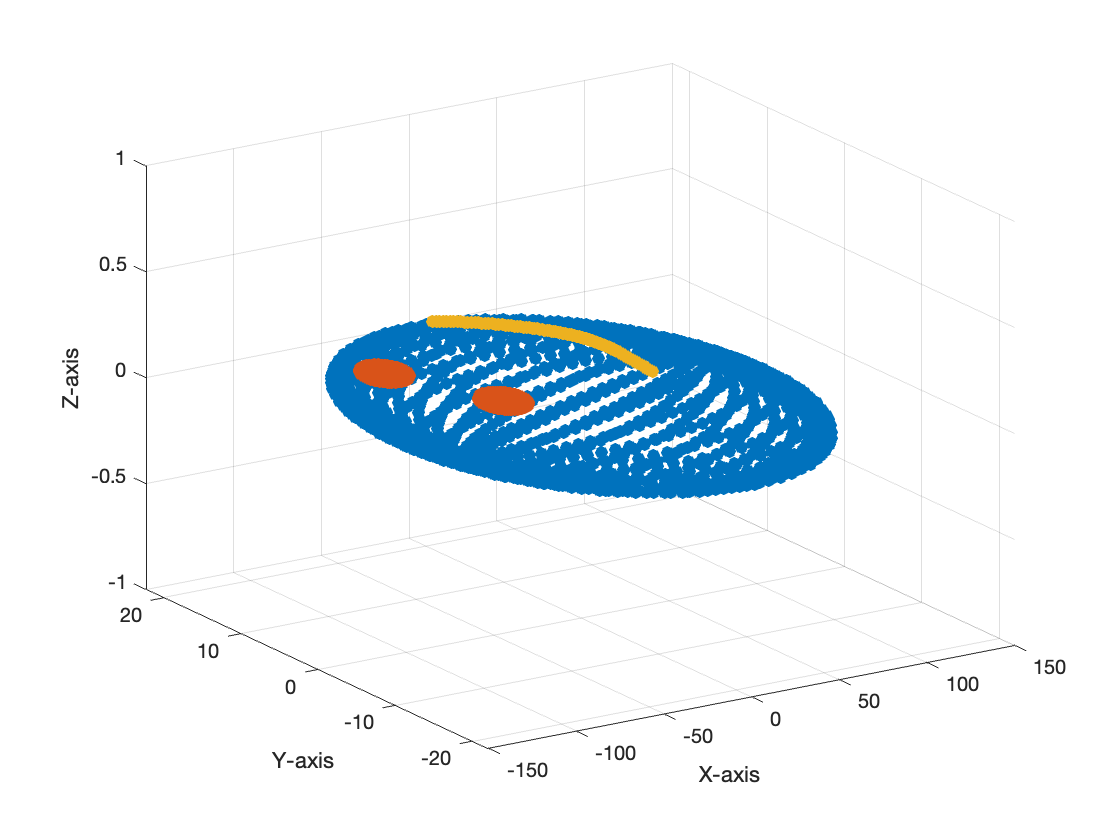
\includegraphics[width=29.63cm, height=22.22cm]{face_svd_3D_B_S.png}
\end{center}

This scaled the rotated face in the $x$-direction by a factor of $\answer[tolerance=.01]{10.4962}$, in the $y$-direction by a factor of $\answer[tolerance=.01]{2.1975}$, and in the $z$-direction by a factor of $\answer[tolerance=.01]{0}$.

Notice that the final scaling of the $z$ direction squishes the dimension of the face down to $\answer{2}$. This accounts for the rank of the matrix $B$, since the result is a $2$D disc (which is about to be rotated by $U$).

Then, we finish by multiplying by $U_B$.

\begin{verbatim}

  two_face=U_B*two_face
  linalg.simple_plot_cloud(two_face)

\end{verbatim}

which yields

%1120x840
\begin{center}
  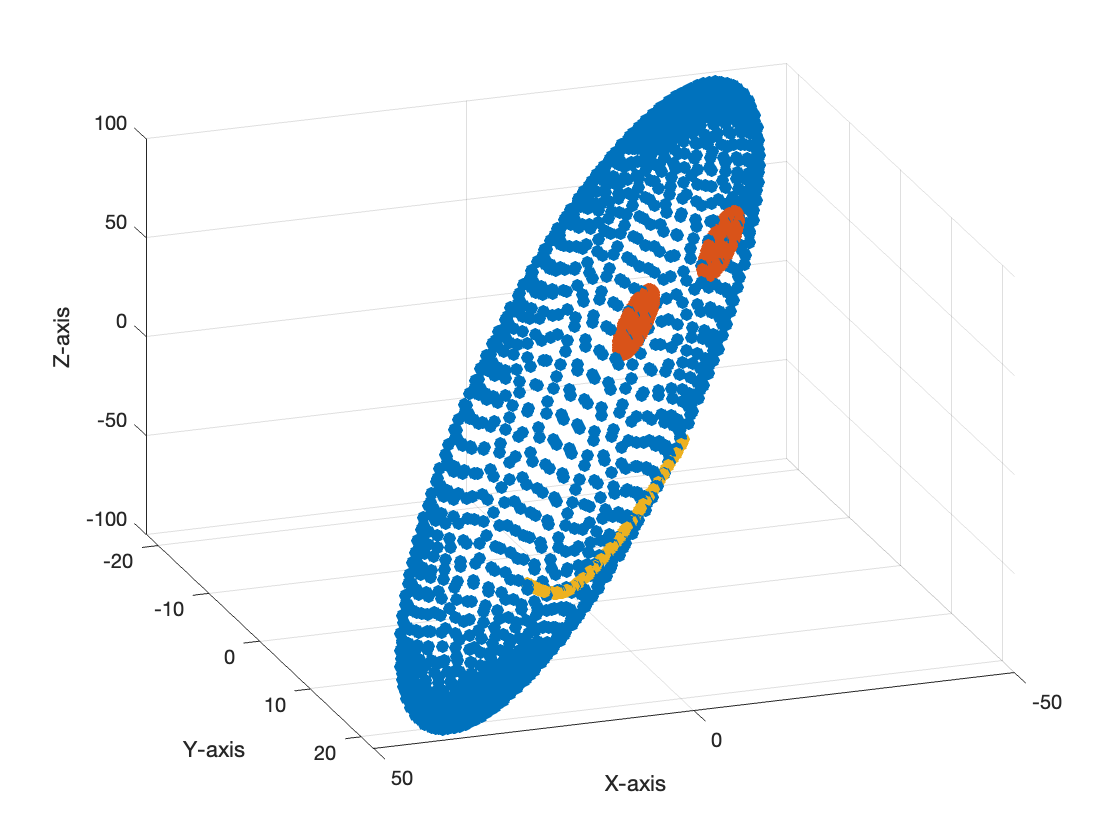
\includegraphics[width=29.63cm, height=22.22cm]{face_svd_3D_B_U.png}
\end{center}

Once again, we have a rotation applied to the disc, and this final transformation matches the result of multiplication by $B$.

This final rotation aligns the face with the following orthonormal basis vectors:

$$u_1=\begin{bmatrix}\answer[tolerance=.001]{.3684}\\\answer[tolerance=.0001]{.2123}\\\answer[tolerance=.0001]{-.9051}\end{bmatrix}, u_2=\begin{bmatrix}\answer[tolerance=.001]{-.9154}\\\answer[tolerance=.0001]{-.0871}\\\answer[tolerance=.0001]{-.3930}\end{bmatrix}, u_3=\begin{bmatrix}\answer[tolerance=.001]{-.1622}\\\answer[tolerance=.0001]{.9733}\\\answer[tolerance=.0001]{.1622}\end{bmatrix}.$$

\end{problem}

What you might notice from this third figure is that the flattened disc is not round and circular, but actually quite stretched in two directions. If you inspect the axes more closely after multiplication by $S_B$, you'll note that this stretching was indeed present, as the $x,y,z$ axes spanned $[-100,100]$, $[-20,20]$ and $[-1,1]$.

\begin{problem}

Based on this analysis, mark which statement is correct about the SVD in this example.

\begin{multipleChoice}

  \choice{$U$ controlled the rank of $B$}
  \choice[correct]{$S$ controlled the rank of $B$}
  \choice{$V$ controlled the rank of $B$}

\end{multipleChoice}

\begin{feedback}

  In fact, you can explain the rank of $B$ by the compressing stage of multiplication by $S$. Since $S$ is diagonal, it stretched and compressed the rotated face matrix along the standard axes. The $x$-direction got stretched by around $10$, the $y$-direction got stretched by around $2$, but the $z$-direction flattened, resulting in a $2$-dimensional disc which was then rotated by $U$. You can in fact describe the process of constructing $B$ from the SVD as: 

  \begin{enumerate}
    \item $V^T$ orthogonally projects data to set up stretching and compression by $S$
    \item $S$ stretches and compresses space according to the rank (and amount of spread) of the matrix (more on this later).
    \item $U$ rotates the stretched and compressed space to the directions over which $B$ spreads image vectors.
  \end{enumerate}

\end{feedback}

\end{problem}

We can actually be even more specific, beyond merely saying $U$ and $V$ rotate and $S$ compresses. There is in fact important and specific information gained by the columns of $U$ and $V$, as well as the diagonal elements of $S$. 

We will adopt specific terminology to refer to these vectors and values. 

\begin{remark}\name{Terminology:}

  The three-matrix decomposition $A=U*S*V^T$ is called the \emph{singular value decomposition} of $A$.
  
  The columns of $U$ are the \emph{left singular vectors}. 

  The columns of $V$ are the \emph{right singular vectors}. 
  
  The diagonal values of $S$ are the \emph{singular values} of a matrix $M$. 
  
  You can for now distinguish the left and right singular vectors by the order of multiplication $U*S*V^T$.
\end{remark}

If you plot the columns of $U$ (the left singular vectors) alongside the final transformation (after scaling for visibility), you get the following 

%1120x840
\begin{center}
  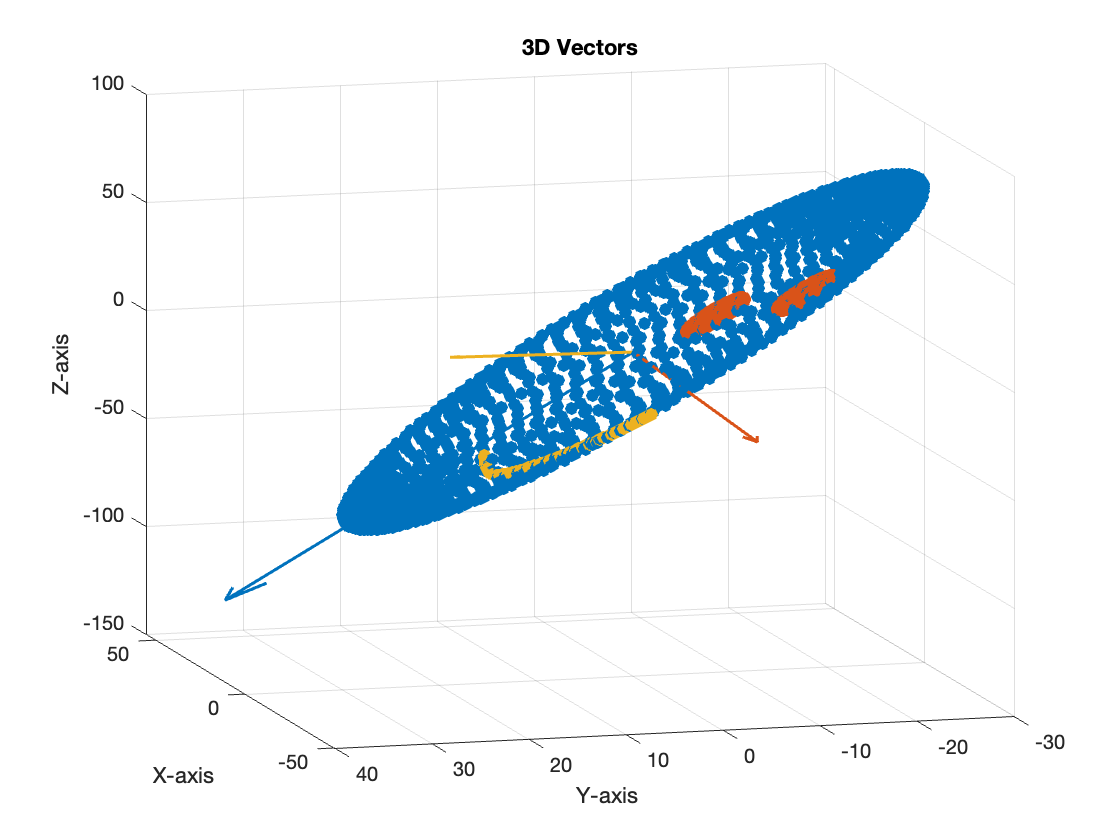
\includegraphics[width=29.63cm, height=22.22cm]{face_svd_B_U_vects.png}
\end{center}

\begin{hint}\name{MATLAB Code}
  \begin{verbatim}

    linalg.simple_plot_cloud(two_face);
    hold on
    linalg.simple_plot_quiver(150*U_B(:,1),50*U_B(:,2),20*U_B(:,3));
    hold off
  
  \end{verbatim}
\end{hint}

The blue vector is the first singular vector, the red is the second, and the yellow is the third. If you plot this yourself and rotate the figure, you'll note that the first two singular vectors orthogonally span the plane on which the disc sits (and hence span the image of the transformation), and the third singular vector is perpendicular to the plane. 

\begin{remark}\name{Looking Ahead: Thinking about Stretching!}

Even more important, the first singular vector points in the direction of the maximum stretching of the disc, the second points in the next direction of stretching, and the third points away from the disc, where there is no stretching. If you return to the singular values (the diagonal of $S$), you actually get a direct correspondance of the amount of stretching (which makes sense, since $S$ stretches and compresses the sphere after rotation by $V$). So the sphere was first stretched by a factor of $10$ (the first singular value) in the $x$-direction, then by a factor of $2$ (the second singular vector) in the $y$-direction, and then by a factor of $0$ (the third singular vector) in the $z$-direction. 

The left singular vectors then rotated space so that the $10$-stretched axis pointed in the direction of $u_1=\begin{bmatrix}.3684\\.2123\\-.9051\end{bmatrix}$, the $2$-stretched axis pointed in the direction of $u_2=\begin{bmatrix}-.9154\\-.0871\\-.3930\end{bmatrix}$, and then the final singular vector points in the direction of the remaining dimension of $3D$ space (the direction over which the vectors were compressed down to the plane).

\end{remark}

All of this lets us utilize the SVD to tell us exactly how any linear transformation re-orients space. If we let a sphere in space (such as \texttt{smiley\_3D}) be a small stand-in for the typical structure of $\RR^3$, we see that all matrices can be described by:

\begin{enumerate}

  \item rotating space to orient along the right singular vectors from $V$
  \item stretching and compressing space along the new axes according to the singular values of $S$ (possibly shrinking the dimension in the case of $0$ singular values)
  \item re-rotating space according to the left singular vectors from $U$

\end{enumerate}

The following video shows this process one more time for the next example.

\begin{center}
  \youtube{SHOfdPSZsSo}
\end{center}

\begin{problem}

Let's explore this with another, non-square matrix, $C=\begin{bmatrix}
  2 & -1 & 1\\
  -6 & 3 & -3
\end{bmatrix}$. 

$C$ is a $2\times 3$ matrix with rank $\answer{1}$, so we anticipate that it will compress $\answer{3}$-dimensional space to a \wordChoice{\choice{point}\choice[correct]{line}\choice{plane}} living in $\answer{2}$-dimensional space. Let's see how the SVD breaks this process down.

First, compute the SVD of $C$ and multiply \texttt{smiley\_3D} by the transposed right singular matrix $V_C^T$.

\begin{verbatim}

  C=[2 -1 1;
      -6 3 -3]
  [U_C,S_C,V_C]=svd(C)
  one_face=V_C'*face
  linalg.simple_plot_cloud(one_face);

\end{verbatim}

%1120x840
\begin{center}
  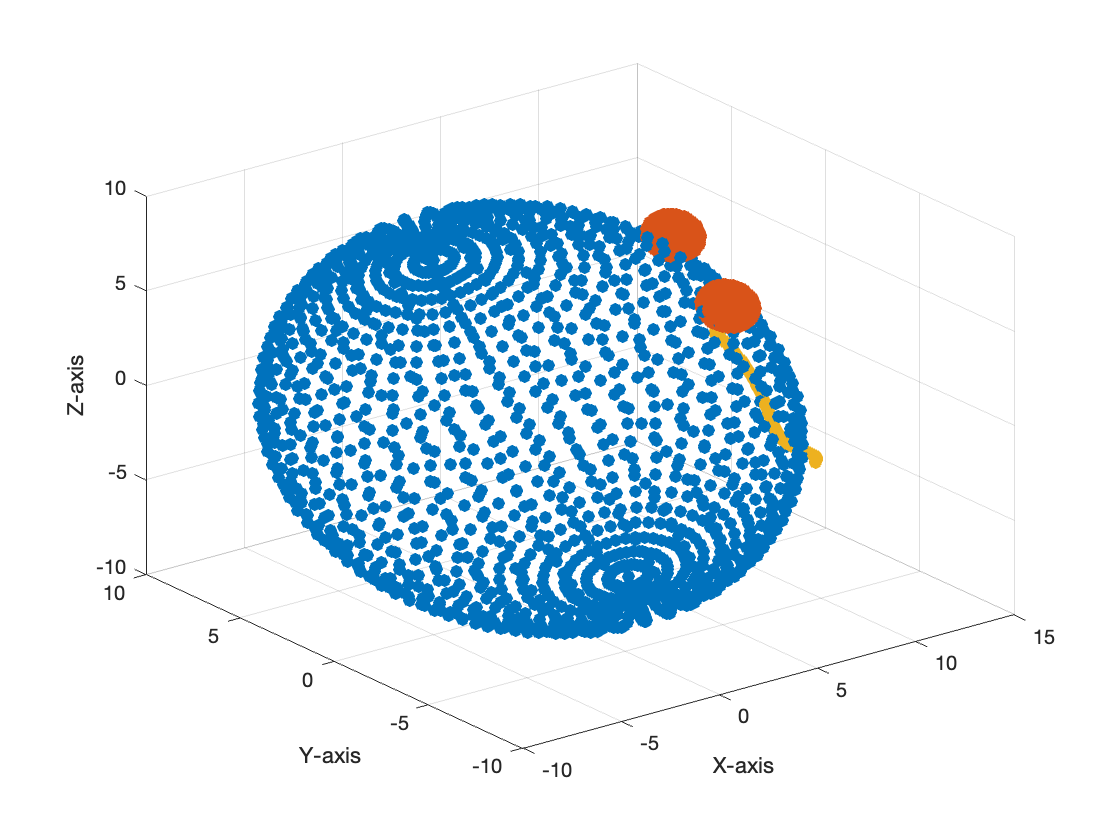
\includegraphics[width=29.63cm, height=22.22cm]{face_svd_C_V.png}
\end{center}

As we can see, this again rotated \texttt{smiley\_3D} in space.

This rotation projects the face vectors to the orthonormal basis vectors:

$$v_1=\begin{bmatrix}\answer[tolerance=.001]{-.8165}\\\answer[tolerance=.0001]{.4082}\\\answer[tolerance=.0001]{-.4082}\end{bmatrix}, v_2=\begin{bmatrix}\answer[tolerance=.001]{.4082}\\\answer[tolerance=.0001]{.9082}\\\answer[tolerance=.0001]{.0918}\end{bmatrix}, v_3=\begin{bmatrix}\answer[tolerance=.001]{-.4082}\\\answer[tolerance=.0001]{.0918}\\\answer[tolerance=.0001]{.9082}\end{bmatrix}.$$

Now, we multiply by $S_C$, the singular value diagonal matrix.


\begin{verbatim}

  one_face=S_C*one_face
  linalg.simple_plot_cloud(one_face);

\end{verbatim}

%1120x840
\begin{center}
  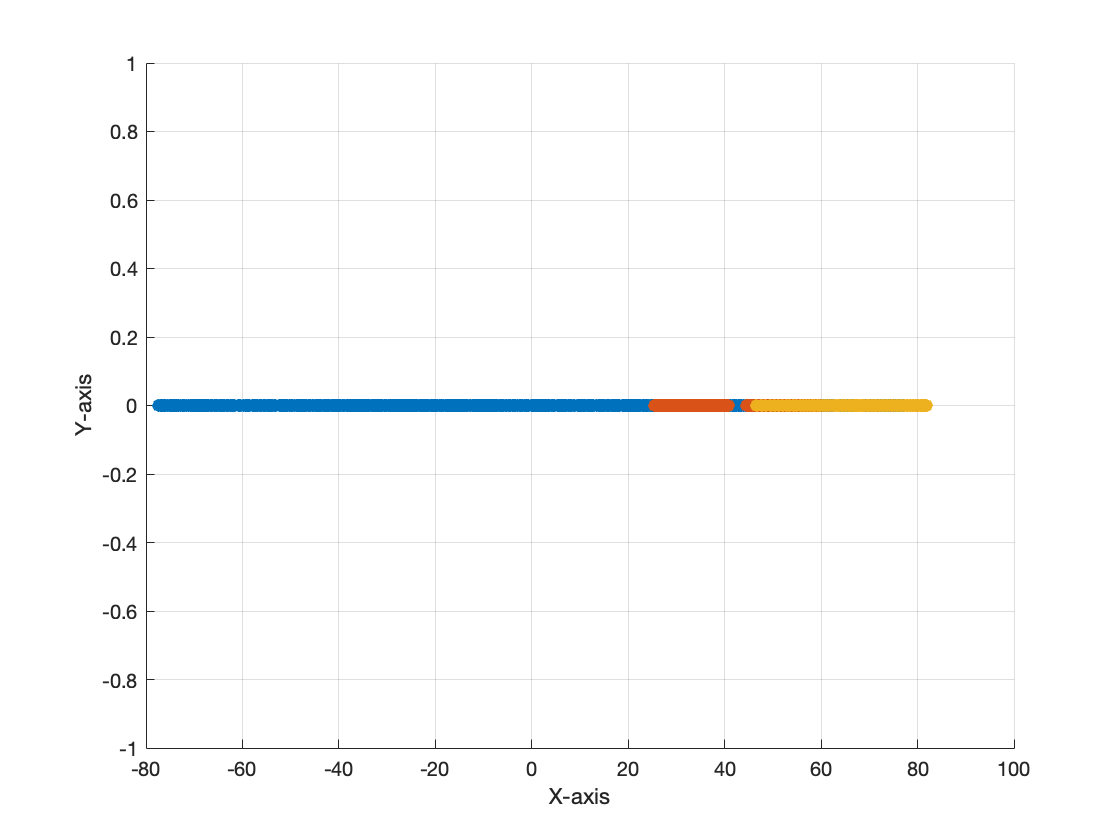
\includegraphics[width=29.63cm, height=22.22cm]{face_svd_C_S.png}
\end{center}

Interestingly, this compressed the face sphere into a line, but a line in $\RR^{\answer{2}}$ rather than in $\RR^3$ as before. This is because $S_C$ transforms $\answer{3}$-dimensional vectors into $\answer{2}$-dimensional vectors but has only $\answer{1}$ nonzero diagonal entry.



 This is in preparation for the left singular matrix $U_C$, which has dimension $2\times 2$, matching the output dimension of the $2\times 3$ matrix. 

Applying the $2$D rotation from the left singular matrix, we get

\begin{verbatim}

  one_face=U_C*one_face
  linalg.simple_plot_cloud(one_face);

\end{verbatim}

%1120x840
\begin{center}
  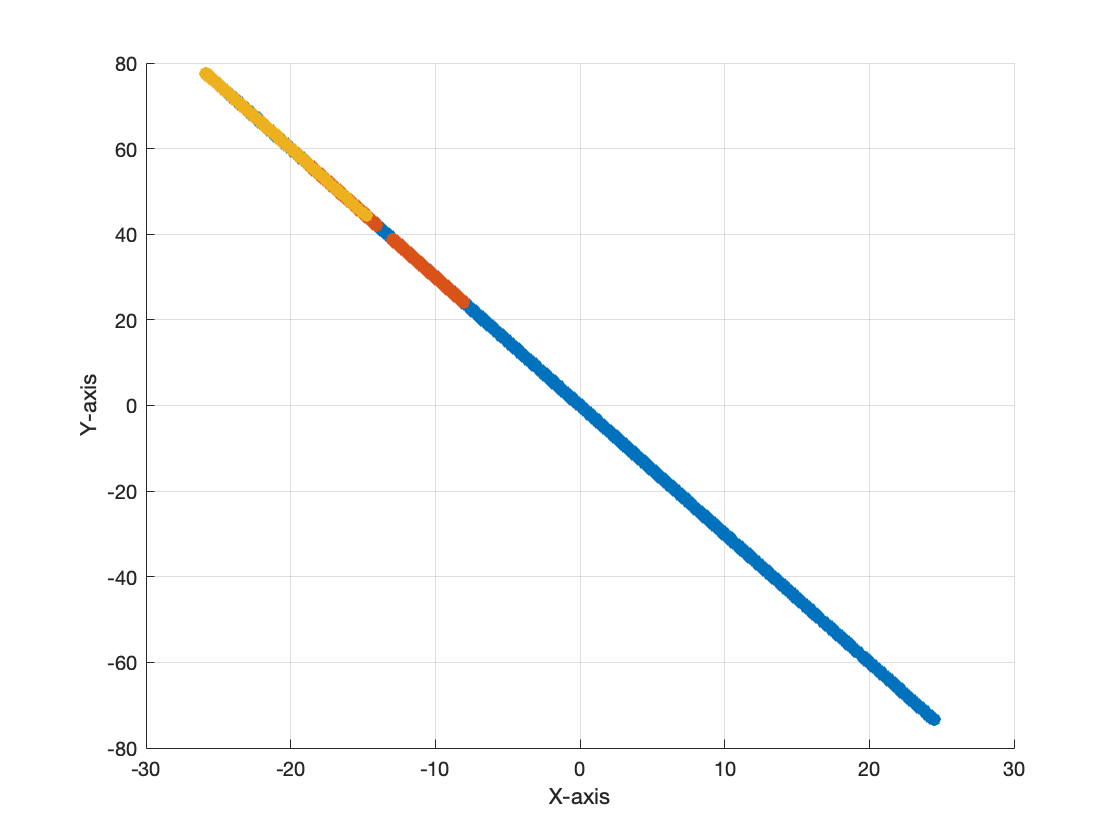
\includegraphics[width=29.63cm, height=22.22cm]{face_svd_C_U.png}
\end{center}

\end{problem}

So, for the matrix $C$, the SVD broke down the rank 1 transformation into a rotation in $3D$ space to align the axes for stretching and compressing, a compression down to a line in $2D$ space, and then a rotation in $2D$ to yeild the final rank 1 $2\times 3$ transformation. 


\begin{problem}

  From the above exploration, and by further exploration in MATLAB, determine which of the following statements are true about the Singular Value Decomposition of an $m\times n$ matrix, $M$. Note, we'll refer to $U$ as an $m\times m$ matrix and $V$ as an $n\times n$ matrix.

  \begin{selectAll}
  
    \choice[correct]{The columns of $U$ are an orthonormal basis for $\RR^m$}
    \choice[correct]{The rank of $M$ is the number of nonzero singular values}
    \choice{The rank of $M$ is the number of singular values}
    \choice{$M$ always has $m$ singular values}
    \choice[correct]{The columns of $V$ are an orthonormal basis for $\RR^n$}
    \choice[correct]{$U$ and $V$ are square matrices in the domain and image space of the transformation from $M$}
    \choice[correct]{The left singular vectors corresponding to nonzero singular values span the image space of $M$}
    \choice[correct]{The right singular vectors corresponding to zero singular values span the kernel of $M$}
    \choice{The left singular vectors corresponding to zero singular values span the image space of $M$}
    \choice{The right singular vectors corresponding to nonzero singular values span the kernel of $M$}
    \choice[correct]{The singular values determine the amount by which the domain space is stretched or compressed (after rotation by $V$)}
    \choice{The singular values determine the amount by which the domain space is stretched or compressed (after rotation by $U$)}

  \end{selectAll}

  \begin{feedback}
  
    Indeed, if you use for loops to iterate through the colums of the singular matrices $U$ and $V$, such as the following

    \begin{verbatim}
      for i=1:3
          for j=1:3
              dot(V_C(:,i),V_C(:,j))
          end
      end
    \end{verbatim}

    you note that the singular vectors form orthonormal bases for $\RR^m$ and $\RR^n$ respectively.

    Further, from the previous two examples, it should be noted that any zero singular vectors entail a reduction of dimension in the image space (because of the flattening along the corresponding axis during multiplication by $S$), so the rank is exactly the number of nonzero singular values. 
    
    Similarly, since $U$ rotates and reflects space according to the left singular vectors, any singular vectors corresponding to nonzero singular values will span the image space of $M$, and any right singular vectors corresponding to zero singular values span the rest of $\RR^m$. Moreover, since $V$ initially projects space to align for the stretching and compression of $S$, the columns of $V$ corresponding to zero singular vectors spans the null space of $M$, since those directions get flattened out by $S$.

  \end{feedback}

\end{problem}

From this exploration, we get the following preliminary definition of the singular value decomposition. We will update this definition as we further explore its properties. First, we must become more concise with our use of ``rotation'' for the singular matrices.

\begin{definition}\name{Orthogonal Matrices}

  A matrix $M$ is \emph{orthogonal} if $M*M^T=I$. 

  In $2$ and $3$ dimensions these correspond to rotations and reflections.

\end{definition}

\begin{definition}\name{Singular Value Decomposition (part 1)}

  The \emph{singular value decomposition} of an $m\times n$ matrix $A$ is a factorization of $M$ into three matrices $U, S$, and $V$ such that $A=U*S*V^T$.

  The matrix $U$ is an orthogonal $m\times m$ matrix whose columns form an orthonormal basis for $\RR^m$. The columns of $U$ are called \emph{left singular vectors}.

  The matrix $V$ is an orthogonal $n\times n$ matrix whose columns form an orthonormal basis for $\RR^n$. The columns of $V$ are called \emph{right singular vectors}.

  The matrix $S$ is diagonal and its diagonal entries are called the \emph{singular values} of $M$

\end{definition}

Now, a theorem capturing the various important properties we've discussed so far about the SVD.

\begin{theorem}\name{Properties of the SVD (part 1)}

  The following are true of the Singular Value Decomposition:

  \begin{enumerate}
    \item The singular value decomposition of any $m\times n$ matrix $A$ always exists.
    \item The left singular vectors $\vec{u}_i$ corresponding to nonzero singular values $\sigma_i$ form a basis for the image space of $A$.
    \item The right singular vectors $\vec{v}_i$ corresponding to zero singular values $\sigma_i$ form a basis for the kernel of $A$.
    \item The rank of $A$ is the number of nonzero singular values. 
    \item The singular values are given in decreasing order.
    \item The singular values correspond to the amount of stretching and compressing in the image space of the matrix $A$ in the directions of the corresponding left singular vectors.
  \end{enumerate}

\end{theorem}

\end{document}